\documentclass[xcolor=table]{beamer}
\usetheme[progressbar=frametitle]{metropolis}
\usepackage{appendixnumberbeamer}

\usepackage[absolute,overlay]{textpos}
\usepackage{booktabs}
\usepackage{pgf, tikz}
\usepackage{pdfcomment}
\usepackage{pgfplots}
\usepackage{hyperref}
\usepackage[utf8]{inputenc}
\usepackage{xspace}
\usepackage{color}
\newcommand{\themename}{\textbf{\textsc{metropolis}}\xspace}
\newcommand\FontImportant{\fontsize{15}{20}\selectfont}
\newcommand\FontMoyenImportant{\fontsize{14}{17}\selectfont}
\newcommand\FontPetit{\fontsize{8}{6}\selectfont}
\title{Simulation de formes réalistes de développement résidentiel, de l'échelle du bâtiment à celle de l'ensemble d'une région urbaine}
\author{Maxime Colomb}
\subtitle{\textit{Sous la direction de M. Brasebin, J. Perret \& C. Tannier}
	\\Soutenance de thèse}

\titlegraphic{\includegraphics[height=1.1cm]{Images/logoIGN.png}\hfill\includegraphics[height=1.1cm]{Images/logoThema.jpg}}

\makeatletter
\newcommand\addsectiontotoc[1]{%
  \addtocontents{toc}{%
    \protect\beamer@sectionintoc{\the\c@section}{#1}{\the\c@page}{\the\c@part}%
                                {\the\beamer@tocsectionnumber}}
}
\makeatother

\makeatletter
\newcommand{\miniscule}{\@setfontsize\miniscule{4}{5}}% \tiny: 5/6
\makeatother

\setbeamerfont*{section in head/foot}{size=\miniscule}
\setbeamercolor{section in head/foot}{parent=palette primary}

\addtobeamertemplate{frametitle}{}{%
  \begin{textblock*}{5cm}(11cm,0.1cm)
    \insertsectionnavigation{4cm}
  \end{textblock*}
}
\begin{document}

\maketitle

\begin{frame}{Contexte : le phénomène d'étalement urbain}
\begin{itemize}
	\item Répond aux souhaits d'un grand nombre de ménages
	\item Multiples effets négatifs
	\item Objectif de régulation
\end{itemize}
\includegraphics[height=2.8cm]{Images/consome.jpg}
\includegraphics[height=2.8cm]{Images/sto.jpeg}
\end{frame}

\begin{frame}{Les différents documents d'aménagement} 
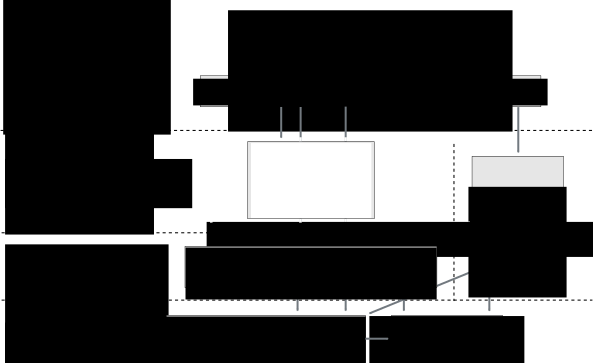
\includegraphics[width=11cm]{Images/planification-globale-Prez.png}
\end{frame}

\begin{frame}{Documents de planification régionale}
Le \textbf{Schéma de Cohérence Territoriale} (SCoT) \textbf{synchronise} les politiques territoriales régionales
\begin{itemize}
\item Territorialise la construction de logements
\item Fixe des contraintes morphologiques et de densité
\end{itemize}
\uncover<2->{Le \textbf{Programme Local de l’Habitat} (PLH) fixe la \textbf{politique du logement}
\begin{itemize}
\item Précise le nombre et le type de logements prévus par communes
\item Programme de futures opérations
\end{itemize}
\uncover<3>{\textbf{Relation de compatibilité entre ces deux documents}}
}
\end{frame}

\begin{frame}{Documents de planification régionale - Exemple}
\includegraphics[width=11cm]{cartes/prevision-plh.png}
\end{frame}

\begin{frame}{Documents de planification locale - Les PLU}
Le \textbf{Plan Local de l’Urbanisme (PLU)} détaille et spatialise les contraintes de constructibilité au sein d’une commune
\begin{itemize}
\item a des \textbf{effets directs sur la constructibilité} mais ne planifie pas la construction 
\item \textbf{donne un cadre} pour la création de programmes de construction de logements \textit{(OAP, ZAC, ZAD)}
\item se compose en partie d'un \textbf{zonage} et d'un \textbf{règlement}
\end{itemize}
\end{frame}	

\begin{frame}{Application d'un PLU - Le zonage}
\begin{columns}[T]
\begin{column}[T]{7cm}
Zones générales et sous-zones particulières
\begin{itemize}
\item \alert{Naturelles} \textbf{(N)} \emph{non constructibles}
\item \alert{Agricoles} \textbf{(A)} \emph{non constructibles}
\item \alert{Urbanisées} \textbf{(U)}
\item \alert{À Urbaniser} \textbf{(AU)}
\end{itemize}
\end{column}
\begin{column}[T]{4cm}
\begin{textblock*}{6cm}(7.5cm,1.5cm)
\includegraphics[width=5cm]{cartes/plu-roche.png}
\end{textblock*}	
\end{column}
\end{columns}

\end{frame}

\begin{frame}{Application d'un PLU - Le règlement}
\begin{columns}[T]
\begin{column}[T]{5cm}
Pour chaque sous-zone : 
\begin{itemize}
\item Articles 1, 2 : restrictions d’\textbf{usage du sol}
\item Articles 6, 7, 8 : \textbf{position des bâtiments} relativement aux autres bâtiments, aux limites de parcelles ou à la voirie
\item Article 10 : \textbf{hauteur maximale}
\item Article 11 : \textbf{aspect extérieur}
\end{itemize}
\end{column}
\begin{column}[T]{5.5cm}
\centering
\includegraphics[width=6cm]{Images/codesplu.png}
\\
\textit{Exemple de prescriptions graphiques (PLU de Strasbourg)}
\end{column}
\end{columns}
\end{frame}

\begin{frame}{Concordance des documents d'urbanisme}
\begin{itemize}
\item Leurs rédacteurs sont différents
\item Leurs objectifs peuvent varier
\item Leurs effets peuvent être contradictoires
\end{itemize}
\uncover<2->{	
\begin{block}{}
\textbf{Nécessité d'uniformiser les documents d'urbanisme et de planification pour que leurs actions soient concordantes}
\end{block}}
\end{frame}

\begin{frame}{Les modèles de simulation spatiale}
\begin{columns}[T]
\begin{column}[T]{7cm}
\begin{block}{}
\textbf{Modélise} un ou plusieurs phénomènes\\

Simulations réapplicables et systématisables\\

\end{block}
\uncover<2->{\begin{block}{}Beaucoup de modèles coexistent\end{block}}
\uncover<3>{\begin{block}{}\textbf{Couplage de modèles existants}\end{block}}
\end{column}
\begin{column}[T]{4cm}

\end{column}
\end{columns}
\end{frame}

\begin{frame}{Problématique : planification régionale -- planification locale}		
	\begin{columns}[T]
	\begin{column}[T]{6cm}
		\begin{block}{}
			\textbf{Scot + PLH : Objectifs de logements
			\\
			PLU : Contraintes de construction
			\\}	
		\end{block}
		\uncover<2->{
			\begin{block}{}
				Comment vérifier la compatibilité entre ces différents documents ?					
			\end{block}	
		}
		
		\uncover<3->{
			\begin{block}{}
				\textbf{Couplage de deux modèles}
				\\
				\uncover<4>{
				Développement résidentiel régional : \textbf{MUP-City} 
				\\
				Constructibilité locale : \textbf{SimPLU} }
			\end{block}
		}	
	\end{column}
	\begin{column}[T]{4cm}
		\only<1>{\includegraphics[width=4.5cm]{Images/final0.png}}
		\only<2-3>{\includegraphics[width=4.5cm]{Images/final1.png}}
		\only<4>{\includegraphics[width=4.5cm]{Images/final2.png}}
	\end{column}
\end{columns}
\end{frame}

\begin{frame}{Enjeux}
	\begin{columns}[T]
		\begin{column}[T]{7cm}
			\begin{block}{}Beaucoup de modèles pour simuler certains aspects du développement résidentiel\end{block}
			\uncover<2>{\begin{block}{}\textbf{Couplage de modèles existants}\end{block}}
	 	\end{column}
	 	\begin{column}[T]{4cm}
	 	\end{column}
	 \end{columns}
\end{frame}

\begin{frame}{Verrous méthodologiques}
	\begin{block}{Fiabilité des modèles de simulation}
	\uncover<2->{{\textit{validation ! calibration ! stabilité ? sensibilité ?}}}
	\end{block}
	\uncover<3->{	
		\begin{block}{Interopérabilité des modèles}
			Différentes échelle\\
			Différents objets\\
			Différentes interprétations\\
			Différentes temporalités\\
		\end{block}
	}
	\uncover<4->{	
		\begin{block}{Données}
			Différentes sources\\
			Différentes granularités\\
		\end{block}		
	}
\end{frame}

\begin{frame}{Objectif de la thèse}
	\begin{block}{}
			Simulation du \textbf{développement résidentiel}
	\end{block}
	\begin{block}{}
			\textbf{Couplage} de deux modèles existants: MUP-City et SimPLU
	\end{block}
\end{frame}
\begin{frame}{Plan de la présentation}
	\begin{itemize}[<+- | alert@+>]
		\item Présentation et analyse de la \textbf{variabilité} de ces deux simulateurs
		\item Présentation d'un \textbf{couplage expérimental}
		\item Application à une commune péri-urbaine
		\item Esquisse d'un outil d'aide à la planification territoriale
	\end{itemize}
\end{frame}

\section[MUP-City]{MUP-City et le développement résidentiel régional}

\begin{frame}{MUP-City}
	\centering{\includegraphics[width=3cm]{Images/mup.png}}
	\\
	Simulation multi-échelle du développement résidentiel 
	\begin{itemize}
		\item Considère une \textbf{région urbaine} entière
		\item Propose une \textbf{organisation spatiale locale}
		\item Met en œuvre différentes \textbf{orientations d'aménagement}
	\end{itemize}
	\includegraphics[width=6.5cm]{Images/ex-sorties-mup.png}
\end{frame}

\begin{frame}{MUP-City: entrées et sorties}
	\textbf{Entrées}
	\begin{itemize}
		\item Environnement vectoriel 
		\item Paramètres de simulation et d'orientations d'aménagements
	\end{itemize}
	\textbf{Sorties}
	\begin{itemize}
		\item \textbf{Cellules de 20m} représentant des emplacements potentiellement urbanisables
		\item Évaluations suivant des critères morphologiques et d'accessibilité
	\end{itemize}
	\begin{block}{}\centering{\includegraphics[width=9.5cm]{Images/schema_mupcity.png}}\end{block}
\end{frame}

\begin{frame}{MUP-City: analyse de sensibilité}
	\begin{itemize}

		\item 	\begin{block}{Étude des variations}
				Réplication de scénario à paramètres égaux : \alert{Robustesse}\\
				Paramètres d'entrée légèrement différents : \alert{Sensibilité}\\
				Choix scénaristiques : \alert{Analyse qualitative}

		
		\end{block}
		\item 	\begin{block}{Objectifs}
				\textbf{Fiabilité} des résultats de simulation\\
				Sélection de \textbf{configurations résidentielles} à exploiter
		\end{block}
	\end{itemize}

	\uncover<2>{\FontPetit\centering\textit{Article en préparation}}\\
	\includegraphics[width=11cm]{Images/ex-sorties-mup2.png}
\end{frame}

\begin{frame}{MUP-City: analyse de sensibilité - Exemples}

\end{frame}

\begin{frame}{Conclusion de cette étude}
	\begin{description}
		\item Systématisation des analyses par la distribution de calculs
		\item Méthodologie reproductible
		\item Sélection de plusieurs sorties à tester dans le couplage\\
	\end{description}
	\begin{block}{}\centering\includegraphics[width=11cm]{Images/exMup.png}\end{block}	
\end{frame}

\section[SimPLU]{SimPLU et la simulation de configurations bâties}

\begin{frame}{Présentation de SimPLU}
	\centering{\textbf{SimPLU}}
	\\
	Génère des configurations bâties en 3D
	\begin{itemize}
		\item Produit un ensemble de configurations potentiellement constructibles selon les \textbf{contraintes du PLU}
		\item Optimise certains paramètres afin de poursuivre différents \textbf{objectifs de construction}
		\item Simule le comportement d'agents constructeurs
	\end{itemize} 
	\centering{\includegraphics[width=5cm]{Images/SimpluOutput.png}}
\end{frame}

\begin{frame}{SimPLU: entrées et sorties}
	\begin{block}{Entrées}
		\begin{itemize}
			\item Parcelle au sein d'un îlot urbain
			\item Dimension et placement des ``boîtes'' simulés
			\item Fonction d'optimisation
		\end{itemize}
	\end{block}
	\begin{block}{Sortie}
		\begin{itemize}
			\item Configuration en 3D représentant un potentiel constructible
		\end{itemize}
	\end{block}
	\begin{block}
		\centering{\includegraphics[width=11cm]{Images/schema_simplu.png}}
	\end{block}		
\end{frame}

\begin{frame}{SimPLU: étude des sorties - Exemple}
	\centering{\includegraphics[width=8.5cm]{Images/simpluOutputSpace.png}}\\
	\FontPetit\centering{\textit{Explorations systématiques visant à la mise au point de de bonnes pratiques pour la création de PLU (Chapron, Brasebin, Perret et al, 2017)}}
\end{frame}

\section[PLUCities]{PLUCities : Couplage de deux modèles de développement résidentiel}

\begin{frame}{Focalisation sur le développement résidentiel}
	\begin{block}{}
		\centering
		\textbf{Objectif :} Contrôler la construction de logements
	\end{block}
	\begin{block}{}

	\end{block}
\end{frame}

\begin{frame}{Documents de planification régionale}
	Le \textbf{Schéma de Cohérence Territoriale} (SCoT) \textbf{synchronise} les politiques territoriales régionales
	\begin{itemize}
		\item Territorialise la construction de logements
		\item Fixe des contraintes morphologiques et de densité
	\end{itemize}
	\uncover<2->{Le \textbf{Programme Local de l’Habitat} (PLH) fixe la \textbf{politique du logement}
		\begin{itemize}
			\item Précise le nombre et le type de logements prévus par communes
			\item Programme de futurs opérations
		\end{itemize}
		\uncover<3>{\textbf{Relation de compatibilité entre ces deux documents}}
	}
\end{frame}

\begin{frame}{Documents de planification régionale - Exemple}
	\includegraphics[width=10.5cm]{cartes/prevision-plh.png}
\end{frame}

\begin{frame}{Documents de planification locale - Les PLU}
	Le \textbf{Plan Local de l’Urbanisme (PLU)} détaille et spatialise les contraintes de constructibilité au sein d’une commune
	\begin{itemize}
		\item a des \textbf{effets directs sur la constructibilité} mais ne planifie pas la construction 
		\item \textbf{donne un cadre} pour la création de programmes de construction de logements \textit{(OAP, ZAC, ZAD)}
		\item se compose en partie d'un \textbf{zonage} et d'un \textbf{règlement}
	\end{itemize}
\end{frame}	

\begin{frame}{Application d'un PLU - Le zonage}
	\begin{columns}[T]
		\begin{column}[T]{7cm}
			Zones générales et sous-zones particulières
			\begin{itemize}
				\item \alert{Naturelles} \textbf{(N)} \emph{non constructibles}
				\item \alert{Agricoles} \textbf{(A)} \emph{non constructibles}
				\item \alert{Urbanisées} \textbf{(U)}
				\item \alert{À Urbaniser} \textbf{(AU)}
			\end{itemize}
		\end{column}
		\begin{column}[T]{4cm}
			\begin{textblock*}{6cm}(7.5cm,1.5cm)
				\includegraphics[width=5cm]{cartes/plu-roche.png}
			\end{textblock*}	
		\end{column}
	\end{columns}
	
\end{frame}

\begin{frame}{Application d'un PLU - Le règlement}
	\begin{columns}[T]
		\begin{column}[T]{5cm}
			Pour chaque sous-zone : 
			\begin{itemize}
				\item Articles 1, 2 : restrictions d’\textbf{usage du sol}
				\item Articles 6, 7, 8 : \textbf{position des bâtiments} relativement aux autres bâtiments, aux limites de parcelles ou à la voirie
				\item Article 10 : \textbf{hauteur maximale}
				\item Article 11 : \textbf{aspect extérieur}
			\end{itemize}
		\end{column}
		\begin{column}[T]{5.5cm}
			\centering
			\includegraphics[width=6cm]{Images/codesplu.png}
			\\
			\textit{Exemple de prescriptions graphiques (PLU de Strasbourg)}
		\end{column}
	\end{columns}
\end{frame}

\begin{frame}{Concordance des documents d'urbanisme}
	\begin{itemize}
		\item Leurs rédacteurs sont différents
		\item Leurs objectifs peuvent varier
		\item Leurs effets peuvent être contradictoires
	\end{itemize}
	\uncover<2->{	
		\begin{block}{}
			\textbf{Nécessité d'uniformiser les documents d'urbanisme et de planification pour que leurs actions soient concordantes}
		\end{block}}
\end{frame}

\begin{frame}{Le couplage PLUCities}
%\includegraphics[width=9cm]{Images/schema-ectqg-fr.png}\\
	\FontPetit\centering{\textit{Colomb et al, 2017}}
\end{frame}


\begin{frame}{Conclusion sur ce couplage}
	\begin{block}{Conclusion sur cette expérimentation}		
		\begin{itemize}
			\item Couplage expérimental (\textit{conférence ECTQG - août 2017})
			\item \textbf{Différents scénarios} d'extension résidentielle pour un \textbf{même jeu de documents d'urbanisme}
		\end{itemize}
	\end{block}
	\begin{block}{Futurs développements}		
		\begin{itemize}
			\item Approfondir les scénarios
			\item Analyse quantitative
			\item \textbf{Exploration} des différentes configurations spatiales possibles
		\end{itemize}
	\end{block}
\end{frame}

\section{Conclusion}

\begin{frame}{Conclusion sur mes travaux de thèse}
	\begin{block}{Travaux en parachèvement}
		\begin{itemize}
			\item \textbf{Diversité des sorties} de modèles de simulation
			\item \textbf{Couplage} de modèles de simulation produisant des \textbf{développements résidentiels}
			\item Différents paramétrages pour \textbf{orienter} ces développements
		\end{itemize}
	\end{block}
	\begin{block}{Perspectives d'utilisation}
		\begin{itemize}
			\item \textbf{Expérimentation} avec l'agglomération de Besançon (CAGB)
			\item Assistance à la \textbf{révision} des PLU et des PLH (et PLU-H)
			\item \textbf{Auto-génération} de cartes thématiques
			\item \textbf{Couplage} avec des modèles simulant l'évolution du \textbf{marché immobilier}
		\end{itemize}
	\end{block}			
\end{frame}

\begin{frame}{Opportunités pour l'IGN}
%	\centering{\includegraphics[width=4cm]{Images/franceGPU.png}}\\
%	\FontPetit{\textit{Dépôt des PLU sur le GPU}}
	\begin{itemize}
	\item Définition de données adaptées à la simulation des évolutions
	\item Proposition de service aux acteurs de la planification sur l'ensemble du territoire français
	\item Certification de la robustesse du processus de simulation relativement à la qualité des données
	\end{itemize}
\end{frame}

\begin{frame}[standout]
	\centering
	\begin{block}{}	
		\centering	
		Merci pour votre attention
	\end{block}
	\begin{block}{}
		\centering
		\textit{Everything we do is open source}\\
		\large
		\textbf{MUP-City}: \url{https://sourcesup.renater.fr/mupcity/} \\
		\textbf{SimPLU}: \url{https://github.com/IGNF/simplu3D}\\
		\textbf{PLUCities :} \url{https://github.com/maxcolomb/PLUCities}  
	\end{block}
%	\begin{block}{}
%		\centering{Questions?}\\
%		\uncover<2>{\includegraphics[width=7.5cm]{Images/DELAHOUSSE.png}}
%	\end{block}
\end{frame}

\begin{frame}{Données nécessaire à l'éxecution de MUP-City}
	\centering{\includegraphics[width=10cm]{Images/schemaSetData.png}}
\end{frame}
\begin{frame}{Données nécessaire à l'éxecution de SimPLU}
%		\centering{\includegraphics[width=8.5cm]{Images/simplu3DNbConfigs.png}}
%	\centering{\includegraphics[width=5cm]{Images/simplumodel.png}}
\end{frame}
\end{document}
